\documentclass{article}

\usepackage[preprint,nonatbib]{neurips_2024}

\usepackage[utf8]{inputenc}
\usepackage[T1]{fontenc}
\usepackage{hyperref}
\usepackage{url}
\usepackage{booktabs}
\usepackage{amsfonts}
\usepackage{nicefrac}
\usepackage{microtype}
\usepackage{graphicx}
\usepackage{subcaption}
\usepackage{xcolor}

\hypersetup{colorlinks=true, linkcolor=blue, citecolor=blue, urlcolor=blue}

\title{Tiny Recursive Reasoning Models for Industrial\\
Rostering: An Inductive, Verifier-Gated Proposer\\
with Exact-Solver Fallback}

\author{%
  Niraj Pankhania \\
  Coforge \\
  \texttt{niraj.pankhania@coforge.com} \\
}

\begin{document}

\maketitle

\begin{abstract}
Tiny Recursive Models (TRM) and their predecessors (HRM, PTRM) solve hard puzzles
with sub-million-parameter networks by recursing a small core over latent
``reasoning'' and ``answer'' states. To date they have been demonstrated almost
exclusively on puzzle benchmarks (Sudoku, Maze, ARC) and are widely criticised as
\emph{transductive} and narrow, limiting industrial uptake. We present, to our
knowledge, the first measured benchmark of a tiny recursive reasoning model on an
industrial workforce-scheduling task, framed as constraint-based shift rostering.
Our system differs from canonical TRM/PTRM in three ways: it is \emph{inductive}
(no per-instance identity embedding, evaluated on unseen instances); it replaces
the learned Q-head with a \emph{deterministic verifier} for inference-time
best-of-$N$ selection; and it wraps the proposer in an \emph{exact-solver
fallback} (OR-Tools CP-SAT), making the deployed system sound by construction. On
commodity CPU we reproduce the central TRM claim---recursion with deep
supervision is the performance driver at fixed parameter count (+23 points on
rostering)---and show verifier-gated scaling reaching 91.5\% feasibility while the
Q-head plateaus near 82\%. The verifier-gated hybrid attains 100\% feasibility
while avoiding the exact solver on 89\% of instances and running
$5\times$ faster end-to-end. A multi-seed pilot hardens these results and reports
an honest negative: under a fixed cheap training budget the realised economic
speedup falls with problem size, even though a $\sim$0.2M-parameter recursive
proposer decisively beats an off-the-shelf 0.5B small language model (0\%
feasible, $\sim$30{,}000$\times$ slower per attempt). We conclude the pattern is
\emph{sound and safe} but that its economic case at scale remains to be proven.
\end{abstract}

\section{Introduction}

Recent ``tiny reasoning'' models challenge the assumption that competitive
reasoning requires large models. The Hierarchical Reasoning Model
(HRM)~\cite{hrm}, the Tiny Recursive Model (TRM)~\cite{trm}, and the Probabilistic
TRM (PTRM)~\cite{ptrm} achieve strong results on Sudoku, Maze and ARC with
networks under 10M---sometimes under 1M---parameters by \emph{recursing} a single
small core over two latent states: an evolving answer $y$ and a latent reasoning
state $z$, trained with deep supervision and truncated backpropagation through
time.

Two features have kept these models in the research lab. First, the public
demonstrations are \emph{transductive}: each training instance carries a learned
identity embedding, so the model can only answer instances it has seen, which is
incompatible with most production workflows. Second, the only reported tasks are
abstract puzzles, leaving open whether the mechanism transfers to a constrained
industrial problem with a real cost model.

This paper addresses both. We take the recommended deployment pattern from the
recursive-reasoning literature---a tiny proposer behind a cheap verifier with an
exact-solver fallback---and instantiate it, \emph{inductively}, on workforce
shift rostering: a canonical constraint-satisfaction problem across business
process services, airline crew operations, and financial back-office scheduling.
Our contributions are empirical and applied-systems, not a new architecture:

\begin{enumerate}
\item The first measured benchmark, to our knowledge, of a tiny recursive
reasoning model on an industrial scheduling task (Section~\ref{sec:results}).
\item An \emph{inductive} (identity-free) variant that generalises to unseen
instances, directly addressing the transductivity critique
(Section~\ref{sec:method}).
\item \emph{Verifier-gated} best-of-$N$ selection in place of the learned Q-head,
with the measured gap that justifies it (Section~\ref{sec:scaling}).
\item A quantified proposer-plus-exact-solver hybrid---feasibility, solver-call
reduction, latency---plus a multi-seed pilot that reports both the robustness
wins and an honest economic negative at scale (Section~\ref{sec:pilot}).
\end{enumerate}

\section{Background and Related Work}

\paragraph{Recursive reasoning models.} HRM~\cite{hrm} couples two recurrent
modules at different timescales. TRM~\cite{trm} simplifies this to a single small
network recursed over $(y,z)$ with deep supervision and an EMA of the weights,
outperforming much larger models on ARC-AGI. PTRM~\cite{ptrm} injects Gaussian
noise per recursion step and runs $K$ rollouts, selecting among them with a
learned Q-head. All three are demonstrated on puzzles and use per-instance
identity embeddings, making them transductive.

\paragraph{Neural rostering.} Learning-augmented scheduling is an established
field that we position against but do not supersede. Prior work uses a deep
network to guide branch-and-bound for personnel rostering~\cite{dnntree}, and a
DNN to repair nurse schedules towards feasibility~\cite{nurserepair}. Neither is a
recursive
reasoning model, inductive-by-design, or equipped with verifier-gated test-time
scaling and an exact-solver guarantee.

\paragraph{Our positioning.} Relative to both lines, we contribute a \emph{tiny
recursive} model, trained \emph{inductively}, with \emph{verifier-gated}
inference-time scaling and an \emph{exact-solver fallback} that makes the system
sound by construction, evaluated on feasibility, solver-call reduction and
latency. The underlying primitives (recursion, PTRM-style noise, verifier
best-of-$N$, sound abstention) are from the cited literature; the novelty is their
combination, the inductive setup, and the industrial measurement.

\section{Method}
\label{sec:method}

\paragraph{Model.} We use a single 2-layer MLP-mixer core~\cite{mlpmixer} (the
TRM-MLP variant: token-mixing plus channel-mixing SwiGLU), recursed over two
latent states $y$ (answer logits) and $z$ (latent reasoning). One recursion
\emph{block} performs $n$ latent updates
$z \leftarrow \mathrm{core}(x_\mathrm{emb}, y, z)$ followed by one answer update
$y \leftarrow \mathrm{core}(x_\mathrm{emb}, y, z)$. \emph{Deep recursion} stacks
$T$ blocks with gradient flowing only through the last block (truncated BPTT), and
\emph{deep supervision} applies the loss at each of $N_\mathrm{sup}$ outer steps
with a detached carry. We keep an EMA of the weights and a Q/halt head, as in TRM.
The model has $\sim$221K parameters; a one-pass network with \emph{identical}
parameter count is the ablation control.

\paragraph{Inductive, not transductive.} Unlike TRM/HRM/PTRM we use \emph{no}
per-instance identity embedding---only token and positional embeddings. The model
therefore learns general constraint structure and is evaluated on a held-out set
of instances it never saw; reported accuracy is genuine generalisation.

\paragraph{Verifier-gated inference-time scaling.} Following PTRM we add Gaussian
noise ($\sigma$) to the latent and run $K$ parallel rollouts. We then select the
output with a \emph{deterministic verifier}---the problem's own feasibility
checker---rather than the learned Q-head. For constraint problems a sound verifier
is free.

\paragraph{Verifier-gated hybrid.} At deployment the proposer runs $K$ verifier-
gated rollouts; if none passes, we fall back to an exact CP-SAT
solve~\cite{ortools}. Every returned solution is thus either verifier-passed or
exact---\emph{sound by construction}---so the proposer can only improve cost, never
correctness.

\section{Experimental Setup}

\paragraph{Tasks.} (a) $4\times4$ Sudoku (8 of 16 cells blanked) as a validated CSP
backbone; (b) \textbf{workforce shift rostering}: $6$ workers $\times\,5$ days,
each day requiring exactly 2 day and 1 night shift, a no-night-then-day rest rule,
and at most 4 shifts per worker---the ``fill-the-gap / shift-swap repair'' problem
common in managed-services workforce management. Instances are generated and, in
the fallback path, solved by CP-SAT. Supervised learning requires label-consistent
data, so training instances are filtered to \emph{unique} completions (verified by
CP-SAT solution counting).

\paragraph{Metric and hardware.} The primary metric is \emph{valid-solve /
feasibility rate}: the fraction of held-out instances whose assembled grid passes
the deterministic verifier. All runs are CPU-only (Apple silicon, 4 threads); no
GPU is used.

\section{Results}
\label{sec:results}

\subsection{Recursion with deep supervision is the driver, at equal parameters}

\begin{table}[h]
\centering
\caption{Recursion vs.\ one-pass at \emph{identical} parameter count ($\sim$221K).}
\label{tab:ablation}
\begin{tabular}{lccc}
\toprule
Task & One-pass (same params) & Recursive TRM & Gain \\
\midrule
Sudoku $4\times4$ (8 blanks) & 81.0\% & 99.5\% & +18.5 pp \\
Rostering $6\times5$ (6 blanks) & 58.5\% & 81.5\% & +23.0 pp \\
\bottomrule
\end{tabular}
\end{table}

Both models share architecture and parameter count; the only difference is whether
the core is recursed with deep supervision (Table~\ref{tab:ablation},
Figure~\ref{fig:ablation}). Recursion adds 18--23 points, reproducing on our own
runs the central TRM claim: the gain comes from iterative refinement, not from
parameters.

\begin{figure}[h]
\centering
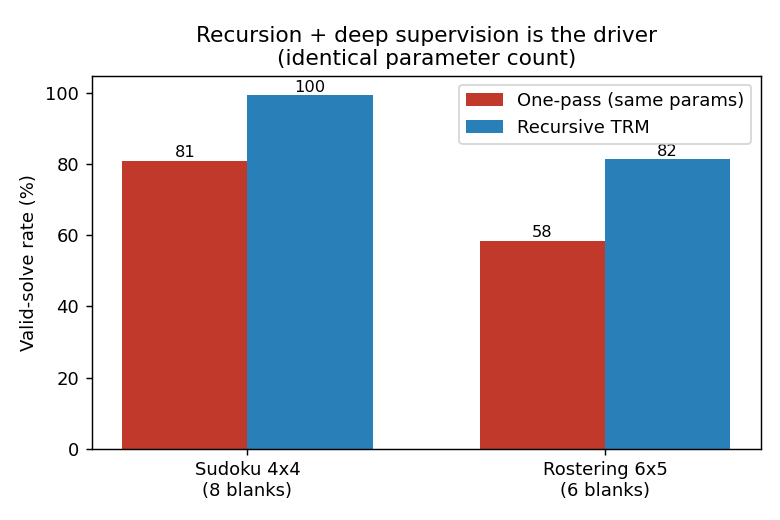
\includegraphics[width=0.52\textwidth]{figs/ablation.png}
\caption{Recursion vs.\ one-pass at equal parameters.}
\label{fig:ablation}
\end{figure}

\subsection{Verifier-gated scaling, and the Q-head ceiling}
\label{sec:scaling}

Adding latent noise and running $K$ rollouts, then selecting with the verifier,
lifts the solve rate with no retraining (Table~\ref{tab:scaling}). Two effects
match the literature. Verifier-gated selection climbs toward the pass@$K$ oracle
(Sudoku reaches 100\%, rostering 91.5\%). Crucially, selection by the \emph{learned
Q-head plateaus well below the verifier}---around 82\% on rostering versus 91.5\%
for the verifier. The operational lesson: do not trust the internal ranking head;
supply a deterministic verifier, which constraint problems natively provide.

\begin{table}[h]
\centering
\caption{Rostering $6\times5$ inference-time scaling (\%). Verifier approaches the
pass@$K$ oracle; the Q-head does not.}
\label{tab:scaling}
\begin{tabular}{lccccc}
\toprule
$K$ & 1 & 4 & 16 & 32 & 64 \\
\midrule
pass@$K$ (oracle) & 81.0 & 87.5 & 90.0 & 91.0 & 91.5 \\
verifier@$K$ & 81.0 & 87.5 & 90.0 & 91.0 & 91.5 \\
Q-head best@$K$ & 81.0 & 81.5 & 82.0 & 79.5 & 79.5 \\
majority@$K$ & 81.0 & 82.5 & 82.0 & 82.0 & 82.0 \\
\bottomrule
\end{tabular}
\end{table}

\begin{figure}[h]
\centering
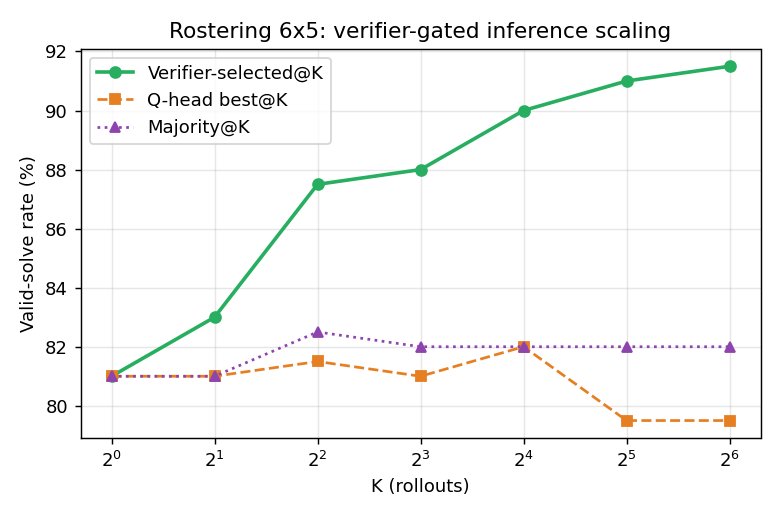
\includegraphics[width=0.52\textwidth]{figs/scaling_roster.png}
\caption{Rostering inference-time scaling: verifier tracks the oracle; the Q-head
plateaus.}
\label{fig:scaling}
\end{figure}

\subsection{The deployable pattern: verifier-gated proposer + exact-solver fallback}

On 200 held-out rostering instances with $K{=}16$ rollouts
(Table~\ref{tab:hybrid}), the hybrid is sound by construction, achieves
\textbf{100\% feasibility}, avoids the exact solver on \textbf{89\%} of instances,
and is \textbf{5.0$\times$ faster} end-to-end than calling CP-SAT every time.

\begin{table}[h]
\centering
\caption{Verifier-gated hybrid on 200 rostering instances ($K{=}16$).}
\label{tab:hybrid}
\begin{tabular}{lccc}
\toprule
Configuration & Feasibility & Solver calls & Total time (200 inst.) \\
\midrule
CP-SAT only (exact) & 100\% & 200 / 200 & 131 ms \\
TRM proposer only & 89.0\% & 0 & 10 ms \\
\textbf{Verifier-gated hybrid} & \textbf{100.0\%} & 22 / 200 & 26 ms \\
\bottomrule
\end{tabular}
\end{table}

\subsection{Scoped pilot: rigor, generalization, economics, and an SLM baseline}
\label{sec:pilot}

The results above are single-seed on a well-trained model. A multi-seed pilot (a
leaner, strictly time-budgeted configuration) hardens them along four axes.

\paragraph{Statistical rigor.} Across 5 seeds on $6\times5$, the proposer's
single-shot valid rate is $48\pm8\%$ and verifier@16 is $59\pm7\%$: a spread wide
enough that any single-seed number must be read as indicative. \emph{Hybrid
feasibility was 100\% on every seed} (Figure~\ref{fig:pilot}a).

\paragraph{Generalization under shift.} Training on 6 blanks and testing harder,
proposer verifier@16 falls $60\%\!\to\!42\%\!\to\!34\%$ at 6/8/10 blanks, yet the
hybrid stays \textbf{100\% feasible} throughout---graceful degradation of
efficiency, never of correctness.

\paragraph{Economics at scale (honest negative).} Per attempt the proposer is
$\sim$7--8$\times$ cheaper than a CP-SAT solve at every size, but the
\emph{realised} hybrid speedup falls with size ($1.92\times\!\to\!1.13\times\!\to\!
0.88\times$ at 30/48/70 cells) because, under a fixed cheap training budget,
proposer accuracy collapses ($48\%\!\to\!28\%\!\to\!2\%$) faster than CP-SAT
slows---so more instances hit the fallback (Figure~\ref{fig:pilot}b).

\paragraph{Off-the-shelf SLM baseline.} On the same $6\times5$ test set, a
general 0.5B small language model~\cite{qwen} prompted few-shot (no fine-tuning)
produced \textbf{0\% feasible} rosters (52\% parse rate) at 3.3 s/instance---over
2{,}000$\times$ more parameters than the recursive proposer, $\sim$30{,}000$\times$
slower per attempt, and unable to do the task (Figure~\ref{fig:pilot}c). A
fine-tuned SLM would be a fairer, stronger baseline and remains future work.

\begin{figure}[h]
\centering
\begin{subfigure}{0.32\textwidth}
  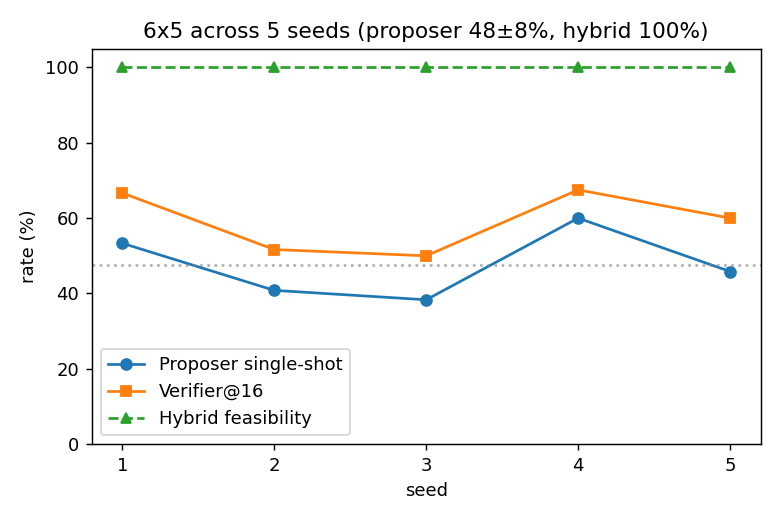
\includegraphics[width=\linewidth]{figs/ws1_seeds.png}
  \caption{Multi-seed ($6\times5$).}
\end{subfigure}\hfill
\begin{subfigure}{0.32\textwidth}
  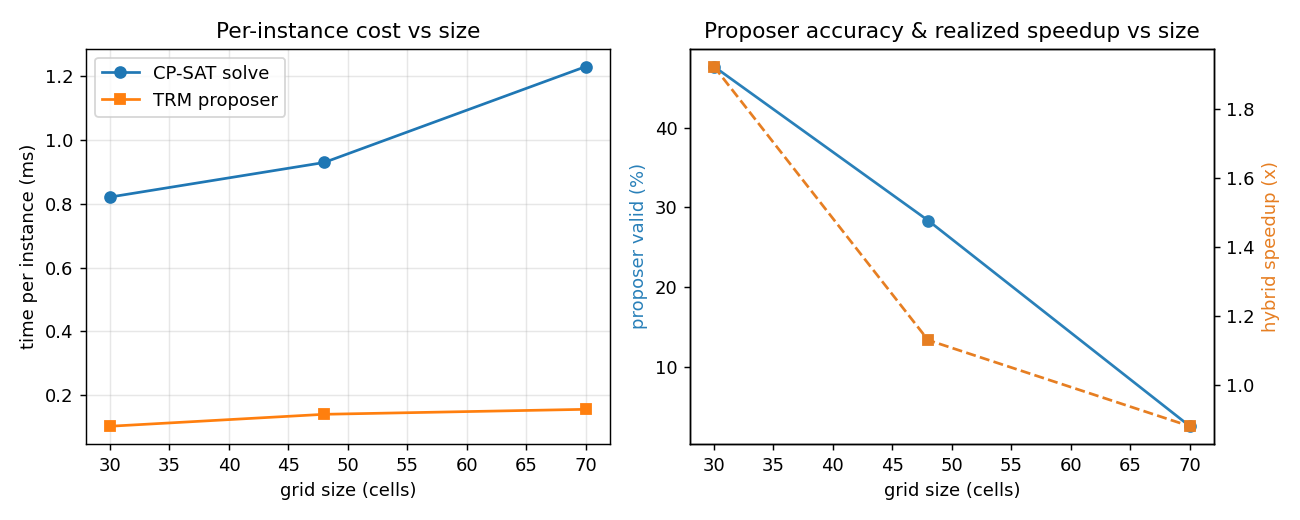
\includegraphics[width=\linewidth]{figs/ws3_size.png}
  \caption{Cost \& speedup vs.\ size.}
\end{subfigure}\hfill
\begin{subfigure}{0.32\textwidth}
  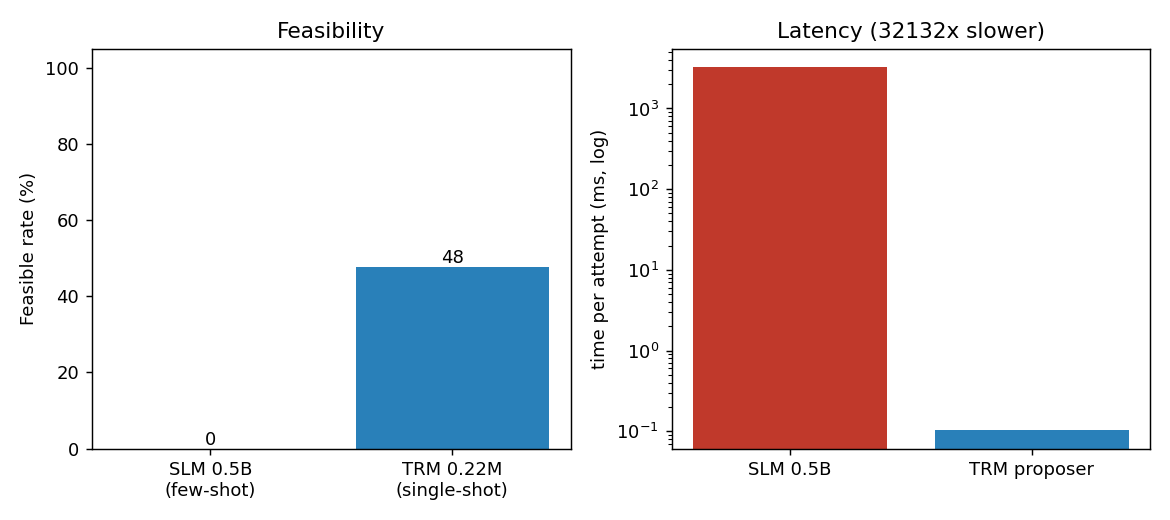
\includegraphics[width=\linewidth]{figs/ws4_slm.png}
  \caption{SLM vs.\ TRM.}
\end{subfigure}
\caption{Pilot. (a) Hybrid is 100\% feasible on all seeds despite proposer
variance. (b) Per-attempt the TRM is far cheaper, but realised speedup falls with
size under a cheap budget. (c) A 0.5B SLM is 0\% feasible and orders of magnitude
slower.}
\label{fig:pilot}
\end{figure}

\paragraph{Verdict.} Against the pre-registered rule (adopt only if the hybrid
beats CP-SAT on cost at matched 100\% feasibility across seeds and sizes):
feasibility and robustness are \emph{met}; cost/latency at scale is \emph{not yet
met}. The mechanism is sound and safe, and beats an off-the-shelf SLM decisively,
but the economic case at scale is unproven under a cheap budget.

\section{Discussion: Industrial Applicability}

The result is about a \emph{reusable pattern}, not rostering specifically. Any
problem that is (i) a fixed-size set of decisions, (ii) governed by cheaply
checkable hard rules, (iii) available in many similar instances, and (iv) under
latency, cost, privacy or edge pressure fits the tiny-proposer + verifier +
exact-solver-fallback architecture. In \textbf{airline operations} this maps onto
crew rostering and pairing, gate/stand assignment, tail assignment, and
disruption recovery (where seconds-scale re-solves are the product). In
\textbf{finance} it fits rule-checking and allocation---trade/order allocation
under position limits, settlement netting and collateral assignment, pre-trade
compliance validation, and desk scheduling. A $\sim$0.2M-parameter model runs on a
laptop or edge device with no cloud dependency, aligning with bank data-residency
and offline airport-operations constraints. Problems needing world knowledge or
continuous optimisation (price prediction, credit decisioning, forecasting,
natural-language handling) are \emph{not} a fit.

\section{Limitations}

Our demonstrations are on small instances (up to $10\times7$); the economic case
at scale is explicitly unproven (Section~\ref{sec:pilot}). Supervised per-cell
training requires label-consistent (unique-completion) data; on the general
many-completion distribution the proposer collapsed to $\sim$2\%, so the
verifier/solver---not the network---guarantees correctness in deployment. The SLM
comparison uses an off-the-shelf model without fine-tuning. The next phase targets
harder, solver-expensive instances, more training per size, multiple seeds
throughout, and a fine-tuned SLM comparator.

\section{Conclusion}

A tiny, inductive recursive reasoning model, gated by a deterministic verifier and
backed by an exact solver, is a credible, CPU-deployable pattern for industrial
constraint satisfaction: it preserves 100\% feasibility, removes most expensive
solver calls, degrades safely under distribution shift, and decisively outperforms
an off-the-shelf small language model. The honest caveat is that its realised
economic advantage at scale is not yet established and is the explicit target of
future work.

\begin{thebibliography}{9}

\bibitem{trm}
A.~Jolicoeur-Martineau.
\newblock Less is More: Recursive Reasoning with Tiny Networks.
\newblock \emph{arXiv:2510.04871}, 2025.

\bibitem{hrm}
G.~Wang et al.
\newblock Hierarchical Reasoning Model.
\newblock \emph{arXiv:2506.21734}, 2025.

\bibitem{ptrm}
Probabilistic Tiny Recursive Model (PTRM).
\newblock \emph{arXiv:2605.19943}, 2026.

\bibitem{dnntree}
Deep-neural-network-guided tree search for personnel rostering.
\newblock \emph{arXiv:2010.14252}, 2020.

\bibitem{nurserepair}
Machine-learning-based repair of nurse schedules.
\newblock \emph{Journal of Advanced Mechanical Design, Systems, and Manufacturing},
2026.

\bibitem{mlpmixer}
I.~Tolstikhin et al.
\newblock MLP-Mixer: An all-MLP Architecture for Vision.
\newblock \emph{NeurIPS}, 2021.

\bibitem{ortools}
L.~Perron and V.~Furnon.
\newblock OR-Tools CP-SAT Solver.
\newblock Google, 2024. \url{https://developers.google.com/optimization}.

\bibitem{qwen}
Qwen Team.
\newblock Qwen2.5 Technical Report.
\newblock \emph{arXiv:2412.15115}, 2024.

\end{thebibliography}

\end{document}
